\chapter{Teknik Pencarian(Search)}

\section{Petunjuk}
\begin{itemize}
	\item Perhatikan petunjuk Dosen untuk berbagai permasalahan Search  !
	\
	\item Perhatikan dan ikuti petunjuk dosen mengenai bagaimana cara menggunakan program Judge untuk mengevaluasi permasalahan yang Anda kerjakan!
\end{itemize}

\pagebreak
\section{Permasalahan}
\begin{permasalahan}{Mama Minta Pulsa}\\
\label{prob:MamaMintaPulsa}
			\begin{figure}[h!]
			\centering
			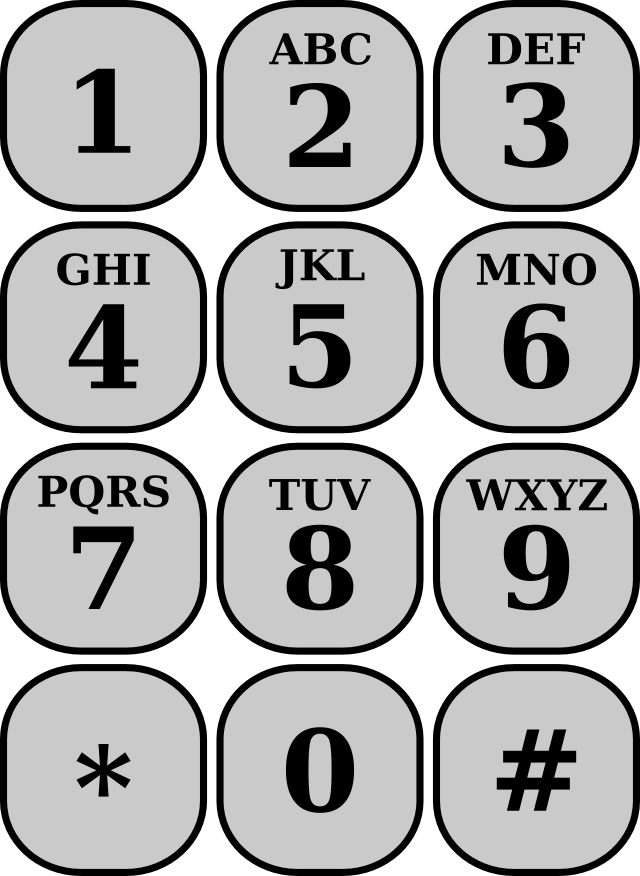
\includegraphics[width=0.5\textwidth]{fig/JamPasir/keypad.png}	
			\end{figure}
	Pernahkah Anda mengirim sms dari era sebelum smartphone ? Untuk membuat sebuah huruf di layar handphone, Anda harus menekan sekumpulan angka berulang - ulang sampai terbentuk sebuah kata. Pada permasalahan ini, Anda diminta untuk menerjemahkan penekanan tombol menjadi kata yang akan terbentuk. Simbol dan huruf besar ada huruf diabaikan, dan angka 0 menyatakan spasi. Semua ouput adalah dalam huruf kecil\\\\
	\textbf{Masukan}\\
	Tipe Data String berupa penekanan tombol\\
	\textbf{Keluaran}\\
	Tipe Data String berupa isi pesan
	\begin{center}
	\textbf{Test Case 1}\\
	\end{center}
	\textbf{Masukan}\\
	6 2 6 2 0 6 444 66 8 2 0 7 88 555 7777 2\\
	\textbf{Keluaran}\\
	mama minta pulsa
	
	\begin{center}
	\textbf{Test Case 2}\\
	\end{center}
	\textbf{Masukan}\\
	6 2 6 2 0 555 2 4 444 0 3 444 0 55 2 66 8 666 777 0 7 666 555 444 7777 444\\
	\textbf{Keluaran}\\
	mama lagi di kantor polisi
	
	\begin{center}
	\textbf{Test Case 3}\\
	\end{center}
	\textbf{Masukan}\\
	5 2 66 4 2 66 0 8 33 555 33 7 666 66 0 6 2 6 2 0 3 88 555 88\\
	\textbf{Keluaran}\\
	jangan telepon mama dulu
	\\\\

\end{permasalahan}


\newpage

\begin{permasalahan}{Sisip !}\\
\label{prob:Sisip}
	Diberikan kumpulan bilangan dan seperangkat instruksi dapatkah Anda menghasilkan posisi terakhir dari instruksi tersebut ? \\
	Kumpulan bilangan akan terdiri dari bilangan bulat, sedangkan perintah akan terdiri dari ``awal``,``akhir`` dan ``samping``. \\
	``Awal`` menyatakan akan ada penempatan data baru di awal.\\
	``Akhir`` menyatakan akan ada penempatan data baru di akhir.\\
	``Samping`` menyatakan ada penempatan data baru di samping dari angka yang ditentukan.
	Setiap angka yang akan disisipkan ke dalam kumpulan bilangan harus unik. \\\\
	\textbf{Masukan}\\
	String berisi : Kumpulan bilangan yang dipisahkan spasi \\
	String berisi : ``perintah`` ``angka yang akan disisipkan`` (``disamping elemen ke``)\\
	\textbf{Keluaran}\\
	Cetakan array paling akhir setelah penyisipan\\
	\begin{center}
	\textbf{Test Case 1}\\
	\end{center}
	\textbf{Masukan}\\
	 1 2 10 4 5 6 7\\
   awal 8\\
	\textbf{Keluaran}\\
	\big[ 8, 1, 2, 10, 4, 5, 6, 7 \big]
	
	\begin{center}
	\textbf{Test Case 2}\\
	\end{center}
	\textbf{Masukan}\\
8 1 2 10 4 5 6 7\\
akhir 8\\
	\textbf{Keluaran}\\
	\big[8, 1, 2, 10, 4, 5, 6, 7\big]

	\begin{center}
	\textbf{Test Case 3}\\
	\end{center}
	\textbf{Masukan}\\
	8 1 2 10 4 5 6 7\\
   akhir 9\\
	\textbf{Keluaran}\\
	\big[8, 1, 2, 10, 4, 5, 6, 7, 9\big] 	 \\\\

	\begin{center}
	\textbf{Test Case 4}\\
	\end{center}
	\textbf{Masukan}\\
	8 1 2 10 4 5 6 7 9\\
   samping 15 2\\
	\textbf{Keluaran}\\
	\big[8, 1, 2, 15, 10, 4, 5, 6, 7, 9\big] 	 \\\\
		

	\begin{center}
	\textbf{Test Case 5}\\
	\end{center}
	\textbf{Masukan}\\
8 1 2 15 10 4 5 6 7 9\\
samping 15 10\\
	\textbf{Keluaran}\\
	\big[8, 1, 2, 15, 10, 4, 5, 6, 7, 9\big] 	 \\\\
	
	
		\begin{center}
	\textbf{Test Case 6}\\
	\end{center}
	\textbf{Masukan}\\
8 1 2 15 10 4 5 6 7 9\\
samping 16 100\\
	\textbf{Keluaran}\\
	\big[8, 1, 2, 15, 10, 4, 5, 6, 7, 9\big] 	 \\\\
	
			\begin{center}
	\textbf{Test Case 7}\\
	\end{center}
	\textbf{Masukan}\\
8 1 2 15 10 4 5 6 7 9\\
samping 20 7\\
	\textbf{Keluaran}\\
	\big[8, 1, 2, 15, 10, 4, 5, 6, 7, 20, 9\big] 	 \\\\
\end{permasalahan}







